\documentclass[10pt]{extarticle}
\usepackage[utf8]{inputenc}
\usepackage{graphicx}
\usepackage{caption}
\usepackage{amsmath}
\usepackage{amssymb}
\usepackage{amsfonts}
\usepackage{tikz}
\usepackage{algorithm}
\usepackage{algpseudocode}

\usetikzlibrary{arrows}
\usetikzlibrary{trees}
\usepackage[a4paper, margin=1cm]{geometry}
\title{Teoria di \textit{Algoritmi e strutture di dati}}
\author{Nicolò Giuliani}
\date{}

\begin{document}
\maketitle
\section*{Analisi del costo Computazionale}
Attraverso il \texttt{Master Threorem} risolviamo ricorrenze del tipo $T(n)=\begin{cases}
  1 \quad n=1 \\
  T(n)=aT(\frac{n}{b})+cn^\beta \quad n>1
\end{cases}$:
\begin{align*}
  \alpha=\frac{\log \,a}{\log \,b} \\
\end{align*}
\begin{itemize}
  \item Se $\alpha > \beta $ allora la complessita' sara' $\Theta(n^\alpha)$
  \item Se $\beta > \alpha $ allora la complessita' sara' $\Theta(n^\beta)$
  \item Se $\alpha = \beta$ allora la complessita' sara' $n^\alpha \log n$
\end{itemize}
\textit{Nota bene}: con $\log$ si intende sempre $\log_2$. \\
\vspace{5px}\\
Ricordiamici di una utile sommatoria notevole:
\begin{align*}
  \sum_{i=0}^n i= \frac{n(n+1)}{2}
\end{align*}
\begin{itemize}
  \item Costo pessimo: O
  \item Costo ottimo: $\Omega$
  \item Costo medio: $\Theta$
\end{itemize}
\section{Liste}
Una lista e' una struttura di dati in cui gli elementi sono ordinati in ordine sequenziale. \\
\begin{figure}[h]
    \centering
    \begin{minipage}[b]{0.3\textwidth}
        \centering
        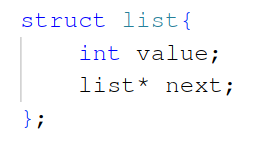
\includegraphics[width=\textwidth]{img/single_linked_list_struct.png}
        \caption{Struttura di una lista singola}
        \label{fig:struct_tree}
    \end{minipage}
    \hspace{0.05\textwidth}
    \begin{minipage}[b]{0.6\textwidth}
        \centering
        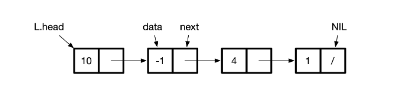
\includegraphics[width=\textwidth]{img/list_foto_single.png}
        \label{fig:albero}
    \end{minipage}
\end{figure} \\
Esiste anche un'altra variante ovvero: Lista doppiamente concatenata \\
\begin{figure}[h]
    \centering
    \begin{minipage}[b]{0.3\textwidth}
        \centering
        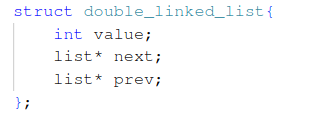
\includegraphics[width=\textwidth]{img/double_list_struct.png}
        \caption{Struttura di una lista doppia}
        \label{fig:struct_tree}
    \end{minipage}
    \hspace{0.05\textwidth}
    \begin{minipage}[b]{0.6\textwidth}
        \centering
        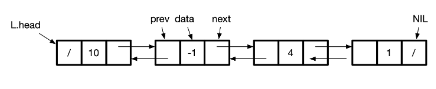
\includegraphics[width=\textwidth]{img/double_list_foto.png}
        \label{fig:albero}
    \end{minipage}
\end{figure} \\
Possiamo trovare anche liste circolari, ovvero che alla fine come puntatore ritorna l'indirizzo del head.
\begin{center}
    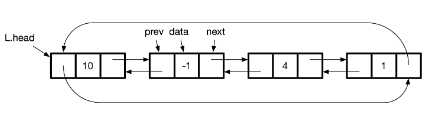
\includegraphics[width=0.6\textwidth]{img/liste_circolari.png}
\end{center} 

\section{Alberi binari}
Un albero è una struttura di dati non-lineare gerarchica.

\begin{figure}[h]
    \centering
    \begin{minipage}[b]{0.6\textwidth}
        \centering
        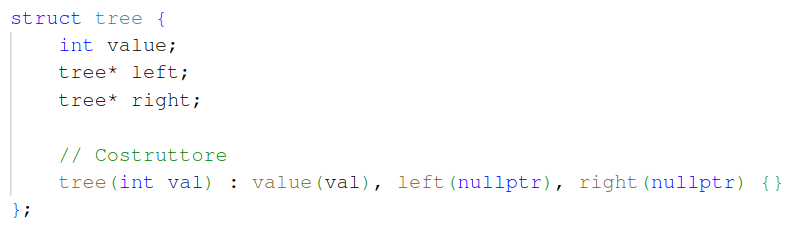
\includegraphics[width=\textwidth]{img/struct_tree.png}
        \caption{Struttura di un albero}
        \label{fig:struct_tree}
    \end{minipage}
    \hspace{0.05\textwidth}
    \begin{minipage}[b]{0.3\textwidth}
        \centering
        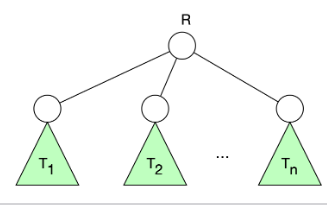
\includegraphics[width=\textwidth]{img/albero.png}
        \caption{Esempio di albero}
        \label{fig:albero}
    \end{minipage}
\end{figure}

In un albero binario ogni nodo puo' avere massimo due figli, si definisce \textit{foglia} il nodo che non ha figli. \\
\begin{itemize}
    \item \textbf{Profondita':} e' la lunghezza di un percorso, unico, che va dalla radice fino ad un nodo specifico, e' sempre log $n$ (con $n$ come foglie totali).
    \item \textbf{Livello:} e' l'insieme di tutti i nodi ad una profondita'.
    \item \textbf{Altezza: } e' la massima profondita', un albero vuoto ha come altezza $-1$.
    \item \textbf{Grado:} numero di figli di un nodo.
\end{itemize}
Si definisce albero binario \textbf{completo} se ogni nodo con figli ne ha 2, mentre i vuoti ne hanno 0. \\
\begin{figure}[h]
    \centering
    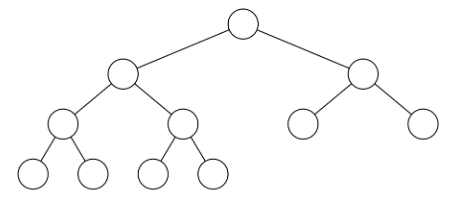
\includegraphics[width=0.3\textwidth]{img/albero_completo.png}
    \caption{Esempio di albero completo}
    \label{fig:etichetta}
\end{figure} \\
Si definisce albero binario \textbf{perfetto} se l'albero e' completo e simmetrico. \\
\begin{figure}[h]
    \centering
    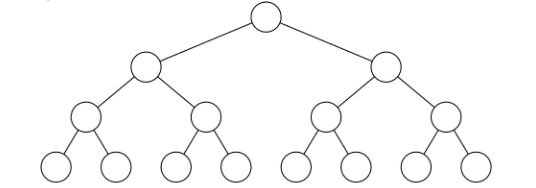
\includegraphics[width=0.3\textwidth]{img/albero_perfetto.png}
    \caption{Esempio di albero perfetto}
    \label{fig:etichetta}
\end{figure} \\
\vspace{5em}
\subsection{Visita di profondità}
\begin{itemize}
    \item \textbf{Pre-ordine}: stampa prima padre, figlio sinistro e poi destro.

    \begin{center}
        \begin{minipage}[b]{0.4\textwidth}
            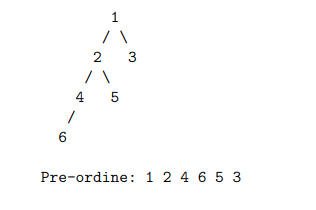
\includegraphics[width=\textwidth]{img/pre_ordine_dati.png}
        \end{minipage}
        \hspace{0.05\textwidth}
        \begin{minipage}[b]{0.4\textwidth}
            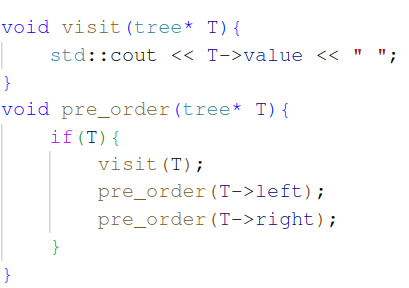
\includegraphics[width=\textwidth]{img/pre_order_tree.png}
        \end{minipage}
    \end{center}

    Costo (ottimo, pessimo, medio): $\Theta(n)$

    \item \textbf{Post-ordine}: stampa prima figlio sinistro, destro, padre.

    \begin{center}
        \begin{minipage}[b]{0.35\textwidth}
            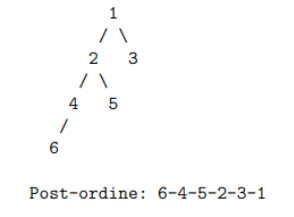
\includegraphics[width=\textwidth]{img/post_ordine_dati.png}
        \end{minipage}
        \hspace{0.05\textwidth}
        \begin{minipage}[b]{0.4\textwidth}
            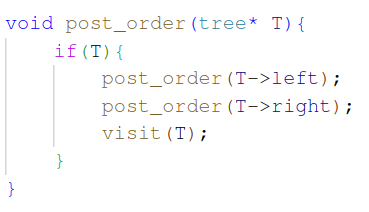
\includegraphics[width=\textwidth]{img/post_order_tree.png}
        \end{minipage}
    \end{center}

    Costo (ottimo, pessimo, medio): $\Theta(n)$

    \item \textbf{In-ordine}: stampa prima figlio sinistro, padre, destro.

    \begin{center}
        \begin{minipage}[b]{0.3\textwidth}
            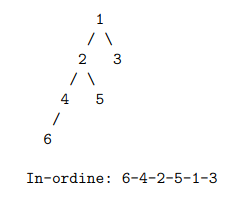
\includegraphics[width=\textwidth]{img/in_ordine_dati.png}
        \end{minipage}
        \hspace{0.05\textwidth}
        \begin{minipage}[b]{0.4\textwidth}
            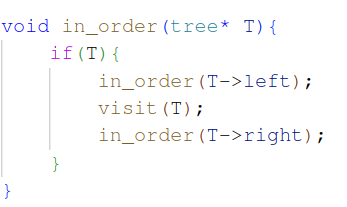
\includegraphics[width=\textwidth]{img/in_order.png}
        \end{minipage}
    \end{center}

    Costo (ottimo, pessimo, medio): $\Theta(n)$
\end{itemize}

\subsection{Visita in ampiezza (livelli)}
Stampa prima padre, poi figlio sinistro, destro e poi sottofigli.
    \begin{verbatim}
        1
       / \
      2   3
     / \
    4   5
   /
  6

In-ordine: 1-2-3-4-5-6
\end{verbatim}
    \begin{center}
        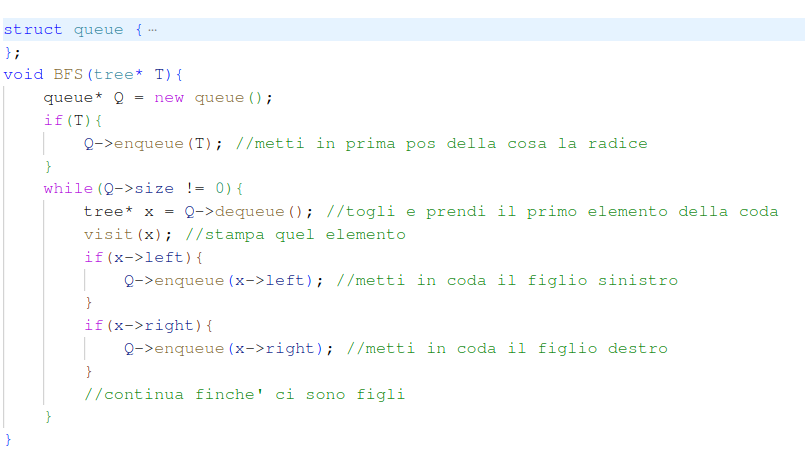
\includegraphics[width=0.8\textwidth]{img/BFS.png}
    \end{center} 
    Costo (ottimo, pessimo, medio): $\Theta(n)$

\subsection{Contare i nodi}
\begin{center}
    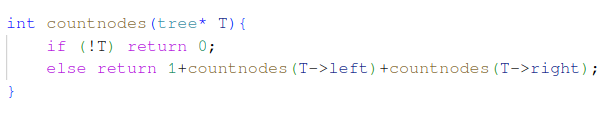
\includegraphics[width=0.6\textwidth]{img/count_nodes_tree.png}
\end{center} 
Costo (ottimo, pessimo, medio): $\Theta(n)$ \\
\vspace{1em} \\
\textit{Nota:} $n$ indica sempre la profondita' dell'albero. 
\pagebreak
\section{Alberi n-ario}
Ovvero un albero con un padre e come figlio una lista di nodi.
\begin{center}
    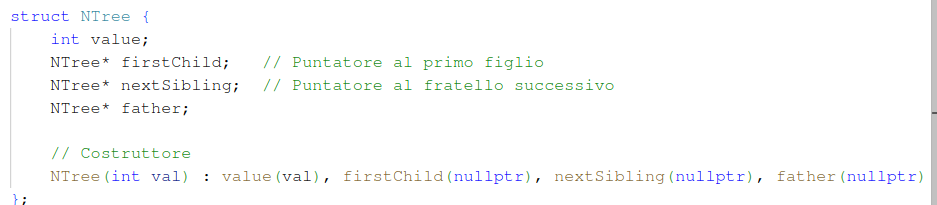
\includegraphics[width=0.9\textwidth]{img/nario_tree.png}
\end{center} 
\begin{figure}[h]
    \centering
    \begin{minipage}[b]{0.4\textwidth}
            \begin{itemize}
                \item Ogni nodo ha un puntatore al primo (\text{first}) figlio
                \item Ogni nodo ha un puntatore al fratello successivo (\text{next})
                \item La lista di figli e' gestita con una lista concatenata sempice
            \end{itemize}
    \end{minipage}
    \hspace{0.05\textwidth}
    \begin{minipage}[b]{0.5\textwidth}
        \centering
        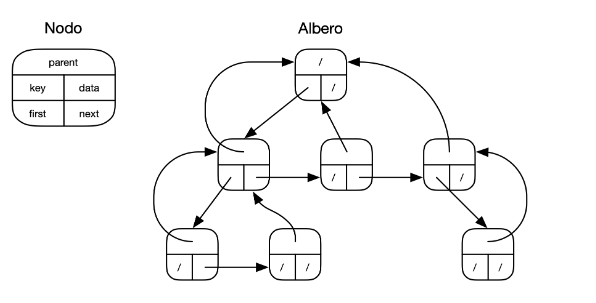
\includegraphics[width=\textwidth]{img/albero_nario_foto.png}
        \caption{Esempio di albero n-ario}
        \label{fig:albero}
    \end{minipage}
\end{figure}
\vspace{2em} 
Esiste anche un'altra versione piu' semplice dove abbiamo un padre e un array di figli di dimensione fissa.
\begin{figure}[h]
    \centering
    \begin{minipage}[b]{0.4\textwidth}
        \begin{center}
            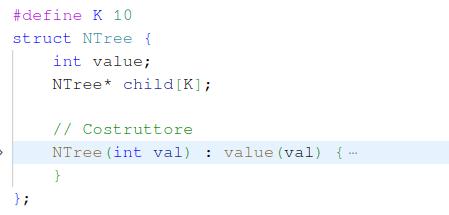
\includegraphics[width=1.4\textwidth]{img/ntree_semplice.png}
        \end{center} 
    \end{minipage}
    \hspace{0.05\textwidth}
    \begin{minipage}[b]{0.5\textwidth}
        \centering
        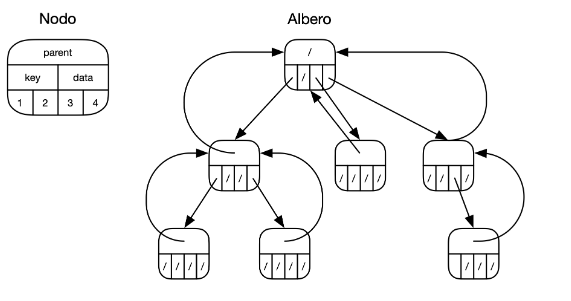
\includegraphics[width=\textwidth]{img/ntree_foto.png}
        \caption{Seconda tipologia di albero n-ario}
        \label{fig:albero}
    \end{minipage}
\end{figure}

\subsection*{Minimax}

Minimax è un algoritmo utilizzato per analizzare alberi di decisione in cui esistono scelte alternative contrastanti tra due agenti o criteri. Nel caso più semplice di massimizzazione, l'algoritmo seleziona il valore massimo possibile lungo i percorsi dell'albero. 

Consideriamo il seguente albero con radice Massimizzante e valori calcolati tramite Minimax:

\[
\begin{tikzpicture}[level distance=1.5cm,
  level 1/.style={sibling distance=5cm},
  level 2/.style={sibling distance=3cm},
  level 3/.style={sibling distance=1.5cm}]
\node {Max}
  child {node {Min}
    child {node {5}}
    child {node {Max}
      child {node {5}}
      child {node {10}}
    }
  }
  child {node {Min}
    child [missing]
    child {node {-1}}
  };
\end{tikzpicture}
\]

\vspace{0.5cm}

\textbf{Passaggi della valutazione Minimax:}

\begin{enumerate}
  \item Riga 1: Max
  \item Riga 2: Min
  \item Riga 3: Max
  \item Riga 4: Min
  \item $\vdots$
\end{enumerate}

\vspace{0.5cm}

\[
\begin{tikzpicture}[level distance=1.5cm,
  level 1/.style={sibling distance=5cm},
  level 2/.style={sibling distance=3cm},
  level 3/.style={sibling distance=1.5cm},
  every node/.style={align=center}]
\node {5 (Max)}
  child {node {5 (Min)}
    child {node {5}}
    child {node {5 (Max)} 
      child {node {5}}
      child {node {10}}
    }
  }
  child {node {-1 (Min)}
    child [missing]
    child {node {-1}}
  };
\end{tikzpicture}
\]
Per gli alberi di minimizzazione si fa: 
\begin{itemize}
  \item min
  \item max
  \item min
  \item max
  \item $\vdots$
\end{itemize}
\subsection*{Alpha-Beta Pruning}

Alpha-Beta Pruning è un miglioramento dell'algoritmo Minimax che permette di ``potare'' (cioè evitare di esplorare) rami dell'albero che non possono influenzare la decisione finale.  
Questo riduce significativamente il numero di nodi da valutare, mantenendo invariato il risultato finale.  

\medskip
Durante la valutazione, si mantengono due valori:
\begin{itemize}
    \item \(\alpha\): il miglior valore (massimo) che il giocatore Max può garantire finora;
    \item \(\beta\): il miglior valore (minimo) che il giocatore Min può garantire finora.
\end{itemize}

Se in un nodo si scopre che \(\beta \leq \alpha\), si può interrompere la valutazione di quel ramo (potatura), perché non influenzerà la scelta finale.


\pagebreak
\section{Alberi binari di ricerca}
Sono alberi binari con la forma: $T.left.value \leq T.value \leq T.right.value$. \\
        \begin{center}
            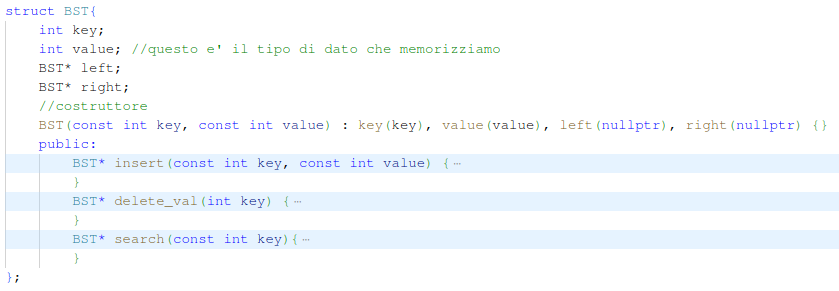
\includegraphics[width=0.8\textwidth]{img/bst_struct.png}
        \end{center} 
Le funzioni elementari sono:
\begin{itemize}
  \item insert(key, value) $\Rightarrow$ inserisce il nuovo nodo e lo ritorna.
  \item delete(key) $\Rightarrow$ elimina il nodo con quella value e lo ritorna.
  \item search(key) $\Rightarrow$ ritorna il nodo con quella value.
\end{itemize}
Complessita': $\Theta(n)$ \\
\vspace{1em} \\
Trovare il massimo e/o il minimo locale/assoluto e' molto semplice:
\begin{center}
    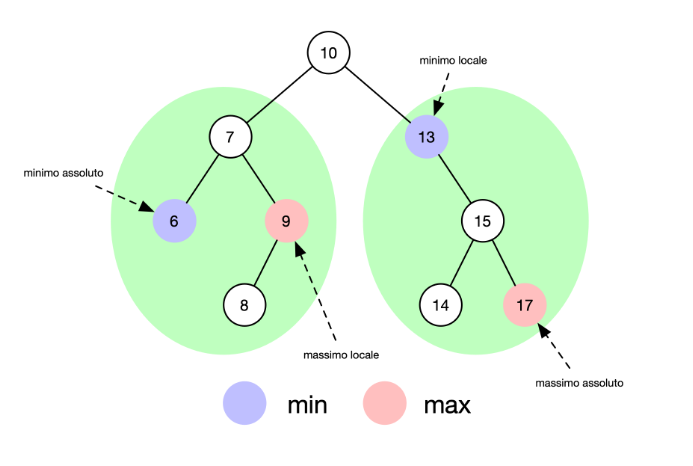
\includegraphics[width=0.5\textwidth]{img/max_min_bst.png}
\end{center} 
Infatti il nodo piu' a sinistra in basso sara' il minimo assoluto, mentre il nodo piu' a destra in basso sara' il massimo assoluto.

\pagebreak
\section{Alberi binari AVL}
Sono alberi binari di ricerca quasi perfetti. \\
\begin{figure}[h]
    \centering
    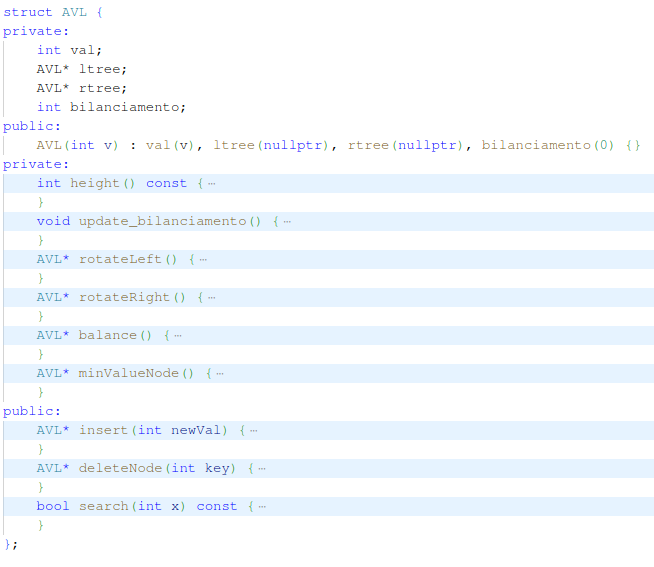
\includegraphics[width=0.6\textwidth]{img/AVL_struct.png}
    \caption{Versione semplificata dove $key=value$}
    \label{fig:etichetta}
\end{figure} \\
Ovvero si calcola con indice $\beta=heigth(ltree)-heigth(rtree)$ e se $\mid\beta\mid \leq 1$ l'abero e' bilanciato.  \\
Quindi l'abero sara' sempre bilanciato in altezza (o quasi perfettamente) dandoci cosi' dei tempi di ricerca delle funzioni di complessita': $\Theta(log \, n)$. \\
Vediamo come l'abero si bilancia:
\begin{itemize}
  \item \textbf{Rotazione a sinistra}
  \[
  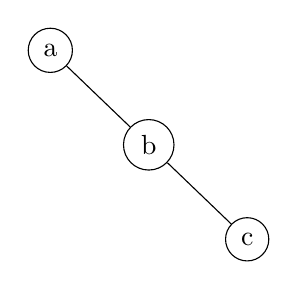
\begin{tikzpicture}[level distance=1.2cm,
    level 1/.style={sibling distance=2.5cm},
    every node/.style={circle,draw}]
  \node {a}
    child[missing]
    child {node {b}
      child[missing]
      child {node {c}}};
  \end{tikzpicture}
  \quad \Rightarrow \quad
  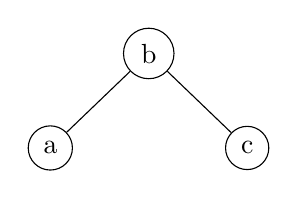
\begin{tikzpicture}[level distance=1.2cm,
    level 1/.style={sibling distance=2.5cm},
    every node/.style={circle,draw}]
  \node {b}
    child {node {a}}
    child {node {c}};
  \end{tikzpicture}
  \]

  \item \textbf{Rotazione a destra}
  \[
  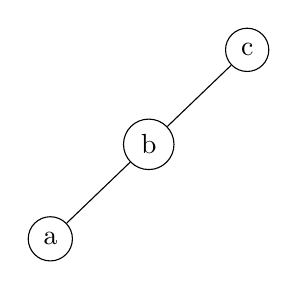
\begin{tikzpicture}[level distance=1.2cm,
    level 1/.style={sibling distance=2.5cm},
    every node/.style={circle,draw}]
  \node {c}
    child {node {b}
      child {node {a}}
      child[missing]}
    child[missing];
  \end{tikzpicture}
  \quad \Rightarrow \quad
  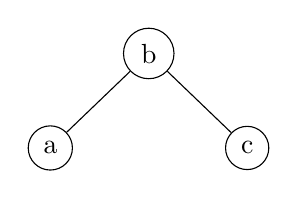
\begin{tikzpicture}[level distance=1.2cm,
    level 1/.style={sibling distance=2.5cm},
    every node/.style={circle,draw}]
  \node {b}
    child {node {a}}
    child {node {c}};
  \end{tikzpicture}
  \]

  \item \textbf{Rotazione sinistra-destra}
  \[
  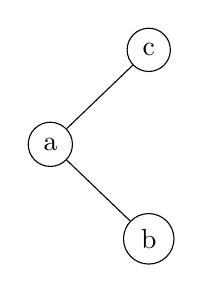
\begin{tikzpicture}[level distance=1.2cm,
    level 1/.style={sibling distance=2.5cm},
    every node/.style={circle,draw}]
  \node {c}
    child {node {a}
      child[missing]
      child {node {b}}}
    child[missing];
  \end{tikzpicture}
  \quad \Rightarrow \quad
  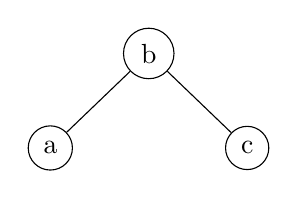
\begin{tikzpicture}[level distance=1.2cm,
    level 1/.style={sibling distance=2.5cm},
    every node/.style={circle,draw}]
  \node {b}
    child {node {a}}
    child {node {c}};
  \end{tikzpicture}
  \]

  \item \textbf{Rotazione destra-sinistra}
  \[
  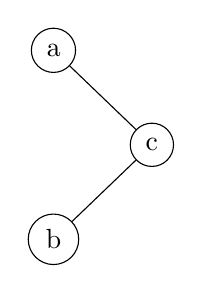
\begin{tikzpicture}[level distance=1.2cm,
    level 1/.style={sibling distance=2.5cm},
    every node/.style={circle,draw}]
  \node {a}
    child[missing]
    child {node {c}
      child {node {b}}
      child[missing]};
  \end{tikzpicture}
  \quad \Rightarrow \quad
  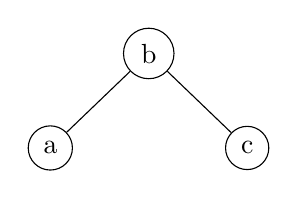
\begin{tikzpicture}[level distance=1.2cm,
    level 1/.style={sibling distance=2.5cm},
    every node/.style={circle,draw}]
  \node {b}
    child {node {a}}
    child {node {c}};
  \end{tikzpicture}
  \]
\end{itemize}
\section{Hash Table}
E' una struttura dati dizionario estremamente efficiente per le funzioniz basilari. \\
\begin{figure}[h]
    \centering
    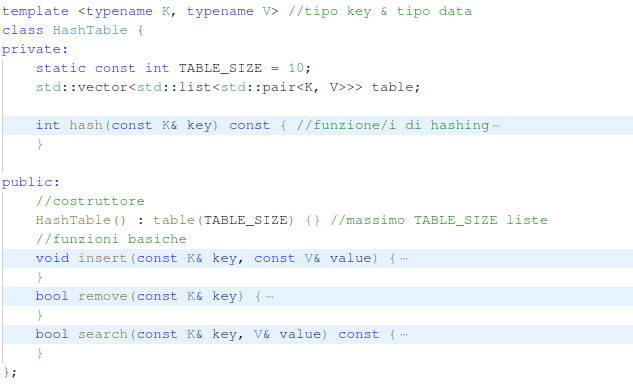
\includegraphics[width=0.6\textwidth]{img/struct_hash.png}
    \caption{Versione dove $K$ indica il tipo di dato della \textit{key} e dove $V$ indica il tipo di dato per il \textit{dato}}
    \label{fig:etichetta}
\end{figure} \\
Per tutte le funzioni basiche abbiamo $\Theta(1)$ ($O(n)$ per insert e search) come costo computazionale. \\
\vspace{1em}
Vediamo la regola generale per hashing basato sulla divisione:
\begin{align*}
  hash(key) \equiv_n key
\end{align*}
\begin{center}
    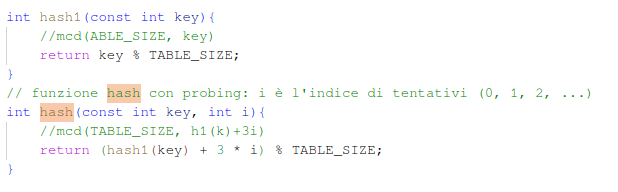
\includegraphics[width=0.8\textwidth]{img/example_has.png}
\end{center}
Ricoda che $x \equiv_n = int(x-n)$, e anche che se $x<n \to x\equiv_n (x)$. \\
\pagebreak
\section{Heap}
\subsection*{BinaryHeap}
E' un albero binario quasi perfetto con $T.val \geq T.child$ (\textit{max-heap}):
\begin{figure}[h]
    \centering
    \begin{minipage}[b]{0.6\textwidth}
       \begin{itemize}
        \item quindi $A.val \geq A.child.cal$ in caso di \texttt{max-heap}
        \item parallelamente abbiamo $A.val \leq A.child.val$ nel \texttt{min-heap}
       \end{itemize}
    \end{minipage}
    \hspace{0.05\textwidth}
    \begin{minipage}[b]{0.3\textwidth}
        \centering
        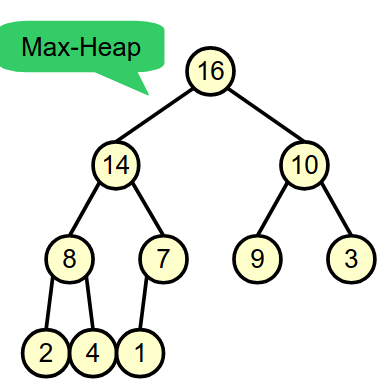
\includegraphics[width=\textwidth]{img/max-heap.png}
        \label{fig:albero}
    \end{minipage}
\end{figure} \\
Abbiamo come funzioni:
\begin{itemize}
  \item $insert()$ costo: $\Theta(\text{log }k)$ (\textit{Attenzione: $k$ indica gli slot occupati dell'array})
\end{itemize}
\subsection*{ArrayHeap}
Possiamo descrivere un BinaryHeap come array:
\begin{figure}[h]
    \centering
    \begin{minipage}[b]{0.3\textwidth}
        \centering
        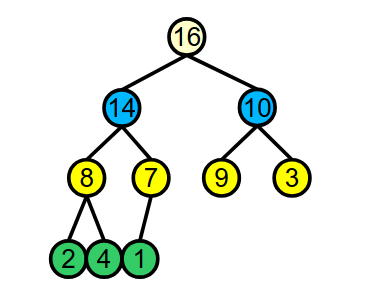
\includegraphics[width=\textwidth]{img/array-heap.png}
        \label{fig:albero}
    \end{minipage}
    \hspace{0.05\textwidth}
    \begin{minipage}[b]{0.3\textwidth}
        \centering
        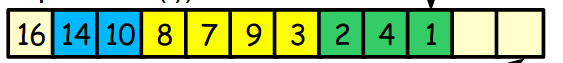
\includegraphics[width=\textwidth]{img/array-heap-lsit.png}
        \label{fig:albero}
    \end{minipage}
\end{figure} \\
Quindi nel array avremo $A[1]$ come genitore, mentre a seguire i figli con visione a livello.
\begin{itemize}
  \item Parent: $A[i]$
  \item Left child: $A[2*i]$
  \item Right child: $A[2*i +1]$
\end{itemize} 
Le funzioni basi (caso max-heap) sono: 
\begin{itemize}
  \item $findMax() \Rightarrow A[1]$, costo di $\Theta(1)$.
  \item $fixHeap()$ sistema la struttura per tornare ad essere un max-heap, costo $\Theta(\text{log} \, n)$. (\textit{attenzione}: la sostituzione e' sempre con il figlio dal valore maggire)
  \item $heapy(\text{int  arr[]})$ dato una array restituisce un array-heap, costo $\Theta(n)$. \\
  Tutorial: si rendono maxHeap (per massimizzare) i figli sx e dx, poi si controlla se $T \geq T.sx$ e se $T \geq T.dx$  e se non e' cosi' si inverte $T$ con il maggiore, poi si applica $fixheap$ sul sottoramo con radice il vecchio $T$.
  \item $deleteMax$ rimuove $A[1]$, costo $\Theta(\text{log} \, n)$. \\
  Tutorial: cancelli $A[1]$ e lo sostituisci con $A[n]$ poi fai fixheap.
\end{itemize}
\textit{Nota:} log $n$ indica come sempre la profindita' dell'abero.
\pagebreak
\section{Union-Find}
Struttura che gestisce insiemi disgiunti. \\
Definiamo \textit{rappresentante} un qualsiasi elemento che ci permette di rappresentare tutto l'insieme.
\begin{center}
    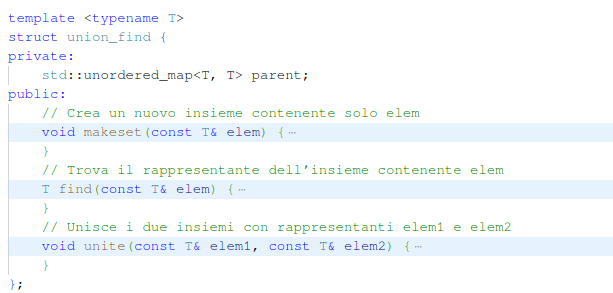
\includegraphics[width=0.6\textwidth]{img/struct-union-find.png}
\end{center}
1) Possiamo descrivere una struttura union-find come un albero di altezza 1:
\begin{figure}[h]
    \centering
    \begin{minipage}[b]{0.3\textwidth}
      \texttt{QuickFind}: struttura con
       \begin{itemize}
        \item makeset() : $O(1)$
        \item find() : $O(1)$
        \item union() : $O(n)$
       \end{itemize}
    \end{minipage}
    \hspace{0.05\textwidth}
    \begin{minipage}[b]{0.35\textwidth}
        \centering
        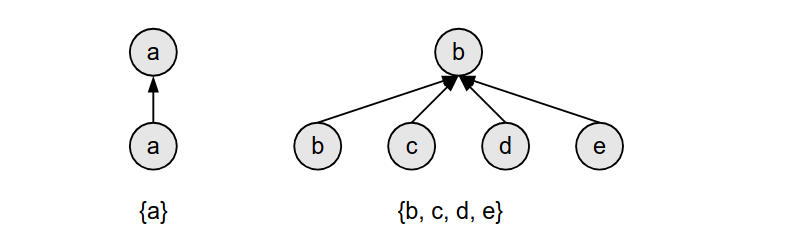
\includegraphics[width=\textwidth]{img/union-find-tree.png}
        \label{fig:albero}
    \end{minipage}
\end{figure} \\
Per ottimizzare il tempo di union() possiamo unire i due insieme con quello che ha piu' elementi come rappresentante (\texttt{euristica sul peso})\\
\begin{center}
    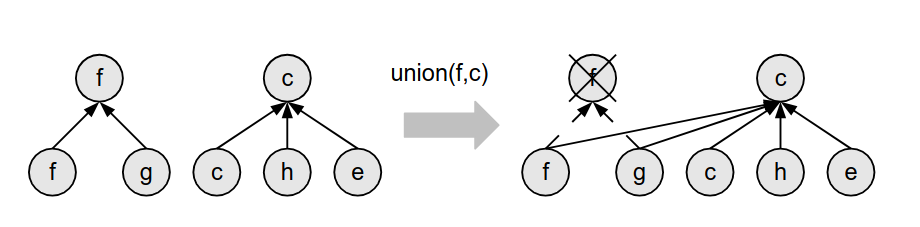
\includegraphics[width=0.6\textwidth]{img/rk.png}
\end{center}
$\Rightarrow \text{union() : }O(\text{log } n)$\\
2) Possiamo anche descrivere union-find come un albergo radicato generico:
\begin{figure}[h]
    \centering
    \begin{minipage}[b]{0.3\textwidth}
      \texttt{QuickUnion}: struttura con
       \begin{itemize}
        \item makeset() : $O(1)$
        \item find() : $O(n)$
        \item union() : $O(1)$
       \end{itemize}
    \end{minipage}
    \hspace{0.05\textwidth}
    \begin{minipage}[b]{0.15\textwidth}
        \centering
        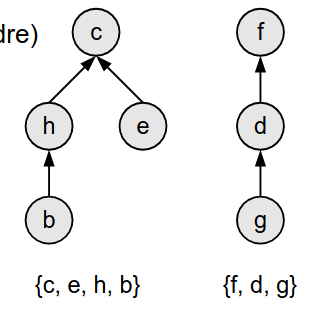
\includegraphics[width=\textwidth]{img/quickunion.png}
        \label{fig:albero}
    \end{minipage}
\end{figure} \\
Per non far diventare gli alberi troppo alti rendiamo la radice dell'albero minore figlia della radice dell'albero maggiore:
\begin{center}
    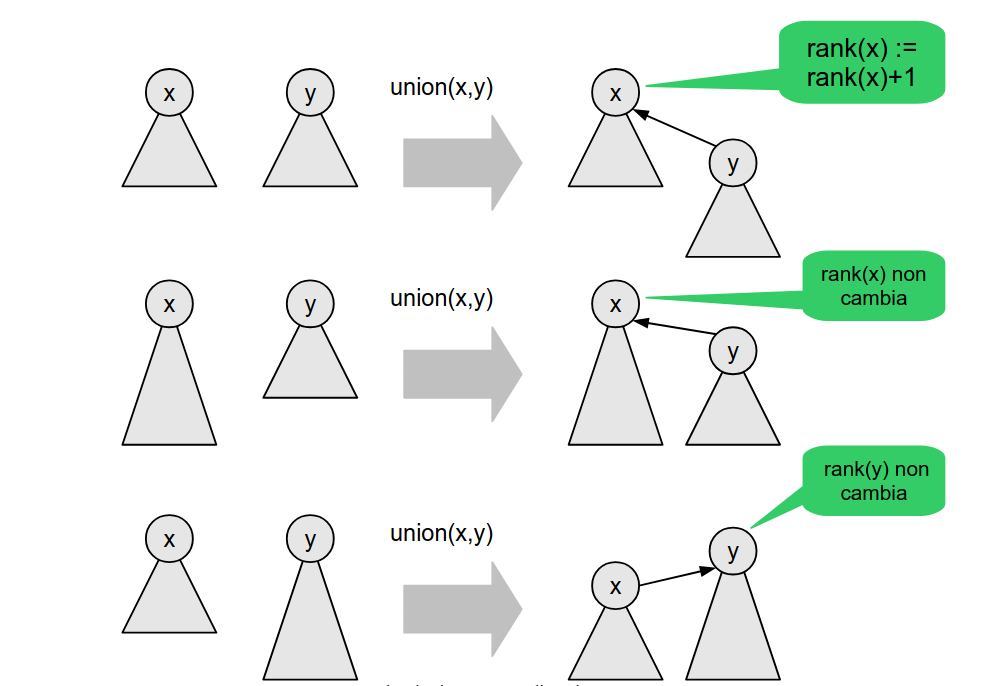
\includegraphics[width=0.4\textwidth]{img/rank.png}
\end{center}
$\Rightarrow \text{find() : } O(\text{log }n)$
\section{Grafi}
E' una struttura matematica dove si rappresentano coppie:
\begin{align*}
  G = (V, E)
\end{align*}
\begin{itemize}
  \item $V$ (vertici) e' l'insieme dei nodi
  \item $E$ (archi) sono le connessioni tra i nodi
\end{itemize}



\begin{figure}[h]
    \centering
    \begin{minipage}[b]{0.4\textwidth}
        \subsection*{Grafo orientato} 
Gli archi hanno direzione \\
\vspace{1em}\\
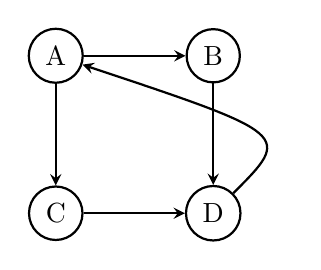
\begin{tikzpicture}[->, >=stealth, node distance=2cm, thick]
  \node[circle, draw] (A) {A};
  \node[circle, draw, right of=A] (B) {B};
  \node[circle, draw, below of=A] (C) {C};
  \node[circle, draw, below of=B] (D) {D};

  \draw (A) -- (B);
  \draw (A) -- (C);
  \draw (B) -- (D);
  \draw (C) -- (D);
  \draw (D) .. controls +(1,1) .. (A); % arco curvo da D ad A
\end{tikzpicture} \\
    \end{minipage}
    \hspace{0.05\textwidth}
    \begin{minipage}[b]{0.4\textwidth}
\subsection*{Grafo non orientato}
Gli archi non hanno direzione \\
\vspace{1em}\\

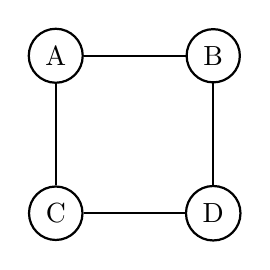
\begin{tikzpicture}[thick]
  \node[circle, draw] (A) {A};
  \node[circle, draw, right of=A, node distance=2cm] (B) {B};
  \node[circle, draw, below of=A, node distance=2cm] (C) {C};
  \node[circle, draw, below of=B, node distance=2cm] (D) {D};

  \draw (A) -- (B);
  \draw (A) -- (C);
  \draw (B) -- (D);
  \draw (C) -- (D);
\end{tikzpicture}\\
    \end{minipage}
\end{figure} 
Un vertice $w$ e' adiacente ad $v$ se e solo se $(w,v) \in E$.
\subsection*{Grafo pesato}
Ad ogni arco si puo' definire un peso (o costo), questo puo' essere definito tramite
\begin{align*}
  c : E \to \mathbb{R}
\end{align*}
Per esempio:  \\
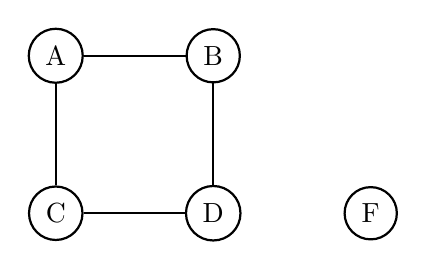
\begin{tikzpicture}[thick]
  \node[circle, draw] (A) {A};
  \node[circle, draw, right of=A, node distance=2cm] (B) {B};
  \node[circle, draw, below of=A, node distance=2cm] (C) {C};
  \node[circle, draw, below of=B, node distance=2cm] (D) {D};
  \node[circle, draw, right of=D, node distance=2cm] (F) {F};
  
  \draw (A) -- (B);
  \draw (A) -- (C);
  \draw (B) -- (D);
  \draw (C) -- (D);
\end{tikzpicture}
\begin{itemize}
  \item $c((A,B))=n \quad (\in \mathbb{R})$
  \item $c(A,F)=\infty$
\end{itemize}
\vspace{1em}
\subsection*{Grado}
definiamolo come il numero di archi che partono da un vertice. \\
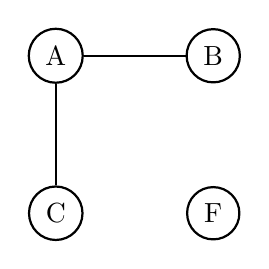
\begin{tikzpicture}[thick]
  \node[circle, draw] (A) {A};
  \node[circle, draw, right of=A, node distance=2cm] (B) {B};
  \node[circle, draw, below of=A, node distance=2cm] (C) {C};
  \node[circle, draw, right of=C, node distance=2cm] (F) {F};
  
  \draw (A) -- (B);
  \draw (A) -- (C);
\end{tikzpicture}
\begin{itemize}
  \item A ha grado 2
  \item B e C hanno grado 1
  \item F ha grado 0
\end{itemize} 
Se si lavora con grafi orientati allora definiamo grado entrante ($e$) e grado uscente ($u$). \\
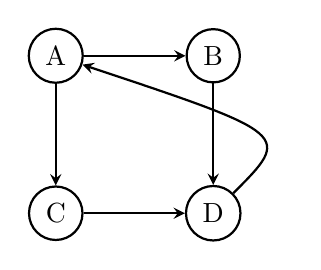
\begin{tikzpicture}[->, >=stealth, node distance=2cm, thick]
  \node[circle, draw] (A) {A};
  \node[circle, draw, right of=A] (B) {B};
  \node[circle, draw, below of=A] (C) {C};
  \node[circle, draw, below of=B] (D) {D};

  \draw (A) -- (B);
  \draw (A) -- (C);
  \draw (B) -- (D);
  \draw (C) -- (D);
  \draw (D) .. controls +(1,1) .. (A); % arco curvo da D ad A
\end{tikzpicture} \\
\begin{itemize}
  \item A ha g.u 2 e ha g.e 1
  \item B, C hanno g.u 1 e g.e 1
  \item D ha g.u 1 e g.e 2
\end{itemize}
Quindi il \textbf{grado} di un vertice e' la somma dei gradi entranti e uscenti di quel vertice.
\subsection*{Cammini}
E' una sequenza di vertici adiacenti per arrivare ad un'altro vertice:
\begin{center}
    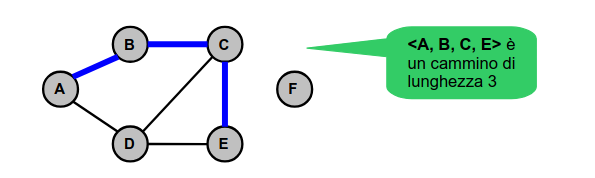
\includegraphics[width=0.6\textwidth]{img/cammino.png}
\end{center}
Questo e' un camino \textbf{semplice}. Si dice cammino \textbf{non} semplice quando dei vertici si ripetono.\\
\vspace{1em}\\
Per la visione dei vertici $v \in V$ possiamo creare una similitudine tra i grafi e gli alberi tali che utilizzando la vista BFS otteniamo
\begin{center}
    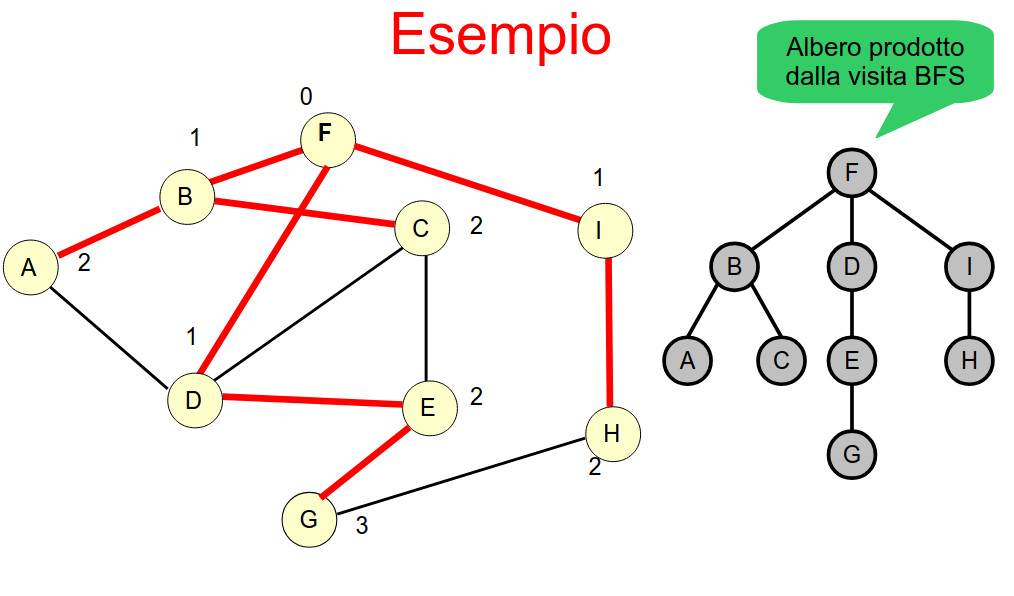
\includegraphics[width=0.6\textwidth]{img/grafoBFS.png}
\end{center}
\textit{Nota:} i numeri sono la distanza tra il vertice radice F e le foglie vertici.
\vspace{1em}\\
Pseudo codice per la visione BFS per i grafi:
\begin{algorithm}
\caption{BFS(Grafo $G=(V,E)$, vertice $v$)}
\begin{algorithmic}[1]
\For{$x \in V$}
    \State $x.\text{visit} \gets \text{false}$
    \State $x.\text{dist} \gets \infty$
\EndFor

\State Queue $q \gets \text{new Queue}()$
\State $v.\text{visit} \gets \text{true}$
\State $v.\text{dist} \gets 0$
\State $q.\text{enqueue}(v)$

\While{not $q.\text{isEmpty}()$}
    \State $u \gets q.\text{dequeue}()$
    \For{$w \in u.\text{adj}()$}
        \If{not $w.\text{visit}$}
            \State $w.\text{dist} \gets u.\text{dist} + 1$
            \State $q.\text{enqueue}(w)$
            \State $w.\text{visit} \gets \text{true}$
        \EndIf
    \EndFor
\EndWhile
\end{algorithmic}
\end{algorithm} \\
\begin{algorithm} 
\caption{hasCycle(G = (V, E))}
\begin{algorithmic}[1]
\State \textbf{Input:} grafo orientato $G = (V, E)$
\State \textbf{Output:} \texttt{true} se $G$ contiene almeno un ciclo, \texttt{false} altrimenti
\ForAll{$v \in V$}
  \State $state[v] \gets 0$ \Comment{$0 =$ non visitato}
\EndFor
\ForAll{$v \in V$}
  \If{$state[v] = 0$}
    \If{\textproc{DFS}($v$)} 
      \State \Return \texttt{true}
    \EndIf
  \EndIf
\EndFor
\State \Return \texttt{false}

\medskip

\Function{DFS}{$u$}
  \State $state[u] \gets 1$ \Comment{$1 =$ in esplorazione}
  \ForAll{$v$ adiacente a $u$}
    \If{$state[v] = 1$} 
      \State \Return \texttt{true} \Comment{ciclo trovato}
    \EndIf
    \If{$state[v] = 0$}
      \If{\textproc{DFS}($v$)} 
        \State \Return \texttt{true}
      \EndIf
    \EndIf
  \EndFor
  \State $state[u] \gets 2$ \Comment{$2 =$ completamente esplorato}
  \State \Return \texttt{false}
\EndFunction
\end{algorithmic}
\end{algorithm} \\
\begin{algorithm}
\caption{Dijkstra(Grafo $G=(V,E,w)$, sorgente $s$, destinazione $d$)}
\begin{algorithmic}[1]
\For{$x \in V$}
    \State $x.\text{dist} \gets \infty$
\EndFor
\State $s.\text{dist} \gets 0$
\State PriorityQueue $Q \gets \text{new PriorityQueue}()$
\State $Q.\text{push}((0, s))$ \Comment{Coppia (distanza, nodo)}

\While{not $Q.\text{isEmpty}()$}
    \State $(\text{currDist}, u) \gets Q.\text{pop\_min}()$ \Comment{Estrai nodo con distanza minima}
    \If{$u = d$}
        \State \textbf{return} $\text{currDist}$ \Comment{Distanza minima trovata}
    \EndIf
    \If{$\text{currDist} < u.\text{dist}$}
        \For{$v \in u.\text{adj}()$}
            \State $\text{alt} \gets u.\text{dist} + w(u,v)$
            \If{$\text{alt} < v.\text{dist}$}
                \State $v.\text{dist} \gets \text{alt}$
                \State $Q.\text{push}((\text{alt}, v))$
            \EndIf
        \EndFor
    \EndIf
\EndWhile

\State \textbf{return} $d.\text{dist}$ \Comment{Se $d$ non raggiungibile sarà $\infty$}
\end{algorithmic}
\end{algorithm}

\pagebreak
\section{Greedy}
\begin{itemize}
  \item Ordina gli elementi secondo un criterio (ad esempio, capacità, valore, tempo di fine).
  \item Scorri gli elementi ordinati e seleziona quelli che soddisfano il vincolo, scegliendo la soluzione localmente ottima in ogni passo.
  \item Alla fine, l’insieme selezionato sarà la soluzione ottima globale (solo se il problema soddisfa il principio di optimalità).
\end{itemize}
\begin{algorithm}
\caption{countDisjointIntervals(array $A[1 \dots n]$)}
\begin{algorithmic}[1]
\State \textbf{Input:} array $A[1 \dots n]$ di coppie $(a_i, b_i)$
\State \textbf{Output:} numero massimo di intervalli disgiunti
\State sort $A$ by $A.second$ crescente
\State int $counter \gets 1$
\State $(last\_start, last\_end) \gets A[1]$
\For{$i = 2$ \textbf{to} $n$}
  \If{$last\_end < A[i].first$}
    \State $(last\_start, last\_end) \gets A[i]$
    \State $counter \gets counter + 1$
  \EndIf
\EndFor
\State \Return $counter$
\end{algorithmic}
\end{algorithm}
\section{Programmazione dinamica}
\subsection{Sottovettore di valore massimo}
Problema: Dato $A[1...n]$ si serca il sottovettore con la somma degli elementi in ordine sia massima
\begin{align*}
  \forall i =1...n\\
  S[i]=max\{\begin{cases}
    V[i] \\
    S[i-1]+V[i]
  \end{cases}\}
\end{align*}
\begin{algorithm}
\caption{sottovettoreMax(int $V[1...n]$)}
\begin{algorithmic}[1]
\State int S[$1 \dots n$];
\State $S[1]=V[1]$
\State int $\text{MaxValue}=S[1]$;
\For{$i = 2$ \textbf{to} $n$}
  \If{$S[i-1] + V[i] > V[i]$}
    \State $S[i] \gets S[i-1] + V[i]$
  \Else
    \State $S[i] \gets V[i]$
  \EndIf
  \If{$S[i] > \text{MaxValue}$}
    \State $\text{MaxValue} \gets S[i]$
  \EndIf
\EndFor
\State \Return $\text{MaxValue}$
\end{algorithmic}
\end{algorithm} \\
Ritorniamo quindi la somma massima di alcuni elementi ordinati di $A$.
\vspace{1em}
\subsection{Problema dello zaino}
Dati $n$ elementi con un peso specifico e un valore specifico, cerchiamo la combinazione massima di valore degli elementi con peso totale inferiore a $K$.\\
Definiamo $V[i, K]$ l'array che simula lo zaino.
\begin{align*}
  \begin{cases}
    V[i,0]=0 \quad \forall i=1\dots n \text{ (ovvero non c'e' uno zaino)}\\
    V[1,K]=v[1] \quad \text{se } K \geq p[1] \text{ (ovvero il primo elemento sta dentro lo zaino)}  \\
    V[1,K]=0 \quad \text{se } p[1] > K \text{ (ovvero il primo elemento NON sta dentro lo zaino)}
  \end{cases}
\end{align*}
Se $p[i] > K$: allora l'elemento $i$ non puo' mai stare dentro lo zaino \\
Se $p[i] \leq K$:
\begin{itemize}
  \item Inseriamo l'oggetto $i$ nello zaino, $V[i, K]=V[i-1, K-p[i]]+v[i]$
  \item Non insieriamo l'oggetto: $V[i, K]=V[i-1, K]$
\end{itemize}
Dato che stiamo massimizzando:
\begin{align*}
  V[i, K]=\text{max}\{\begin{cases}
    V[i-1,K-p[i]]+v[i] \\
    V[i-1, K]
  \end{cases}\}
\end{align*}
Quindi: 
\begin{align*}
  V[i, K]=\begin{cases}
    V[i-1, K] \quad \text{se $p[i] > K$} \\
    \text{max}\{{V[i-1, K-p[i]]+v[i], \, V[i-1, K]}\} \quad \text{se } p[i] \leq K
  \end{cases}
\end{align*} \\
\begin{center}
    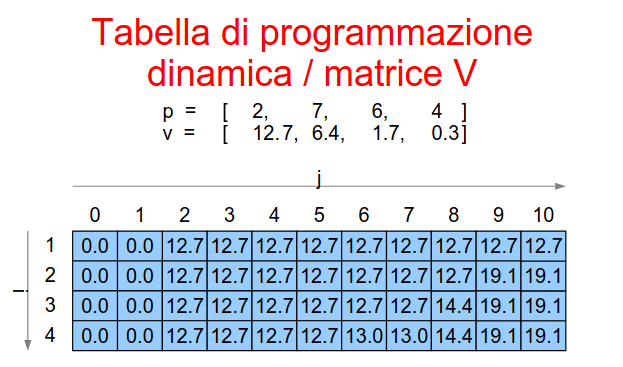
\includegraphics[width=0.6\textwidth]{img/tabella_dinamica.png}
\end{center} 
\begin{algorithm}
\caption{ZainoIntero($v[1..n]$, $p[1..n]$, $K$)}
\begin{algorithmic}[1]
\State int $V[0..n][0..K]$
\For{$i = 1$ \textbf{to} $n$}
  \For{$j = 0$ \textbf{to} $K$}
    \If{$p[i] > j$}
      \State $V[i][j] \gets V[i-1][j]$
    \Else
      \State $V[i][j] \gets \max \big( V[i-1][j], V[i-1][j - p[i]] + v[i] \big)$
    \EndIf
  \EndFor
\EndFor
\State //stampiamo gli indici
\State int $j \gets K$
\For{$i = n$ \textbf{downto} $1$}
  \If{$p[i] \le j$ \textbf{and} $V[i][j] = V[i-1][j - p[i]] + v[i]$}
    \State print($i$)
    \State $j \gets j - p[i]$
  \EndIf
\EndFor
\State \Return $S$
\end{algorithmic}
\end{algorithm} 

\end{document} 